\documentclass{article}
\usepackage[utf8]{inputenc}
\usepackage{booktabs}

\title{Iris replication example}
\author{Erik Buunk}
\date{August 2021}

\usepackage{natbib}
\usepackage{graphicx}

\begin{document}

\maketitle

\section{Introduction}
This is a replication example with the Iris dataset

\section{Results}
The table looks as follows:

\input{../results/tables/my_table}

The result are shown on the next page.

\begin{figure}
    \centering
    \includegraphics[scale=0.35]{../results/figures/r_output.pdf}
    \caption{Plot from R of Iris}
    \label{fig:iris_r}
\end{figure}


\begin{figure}
\centering
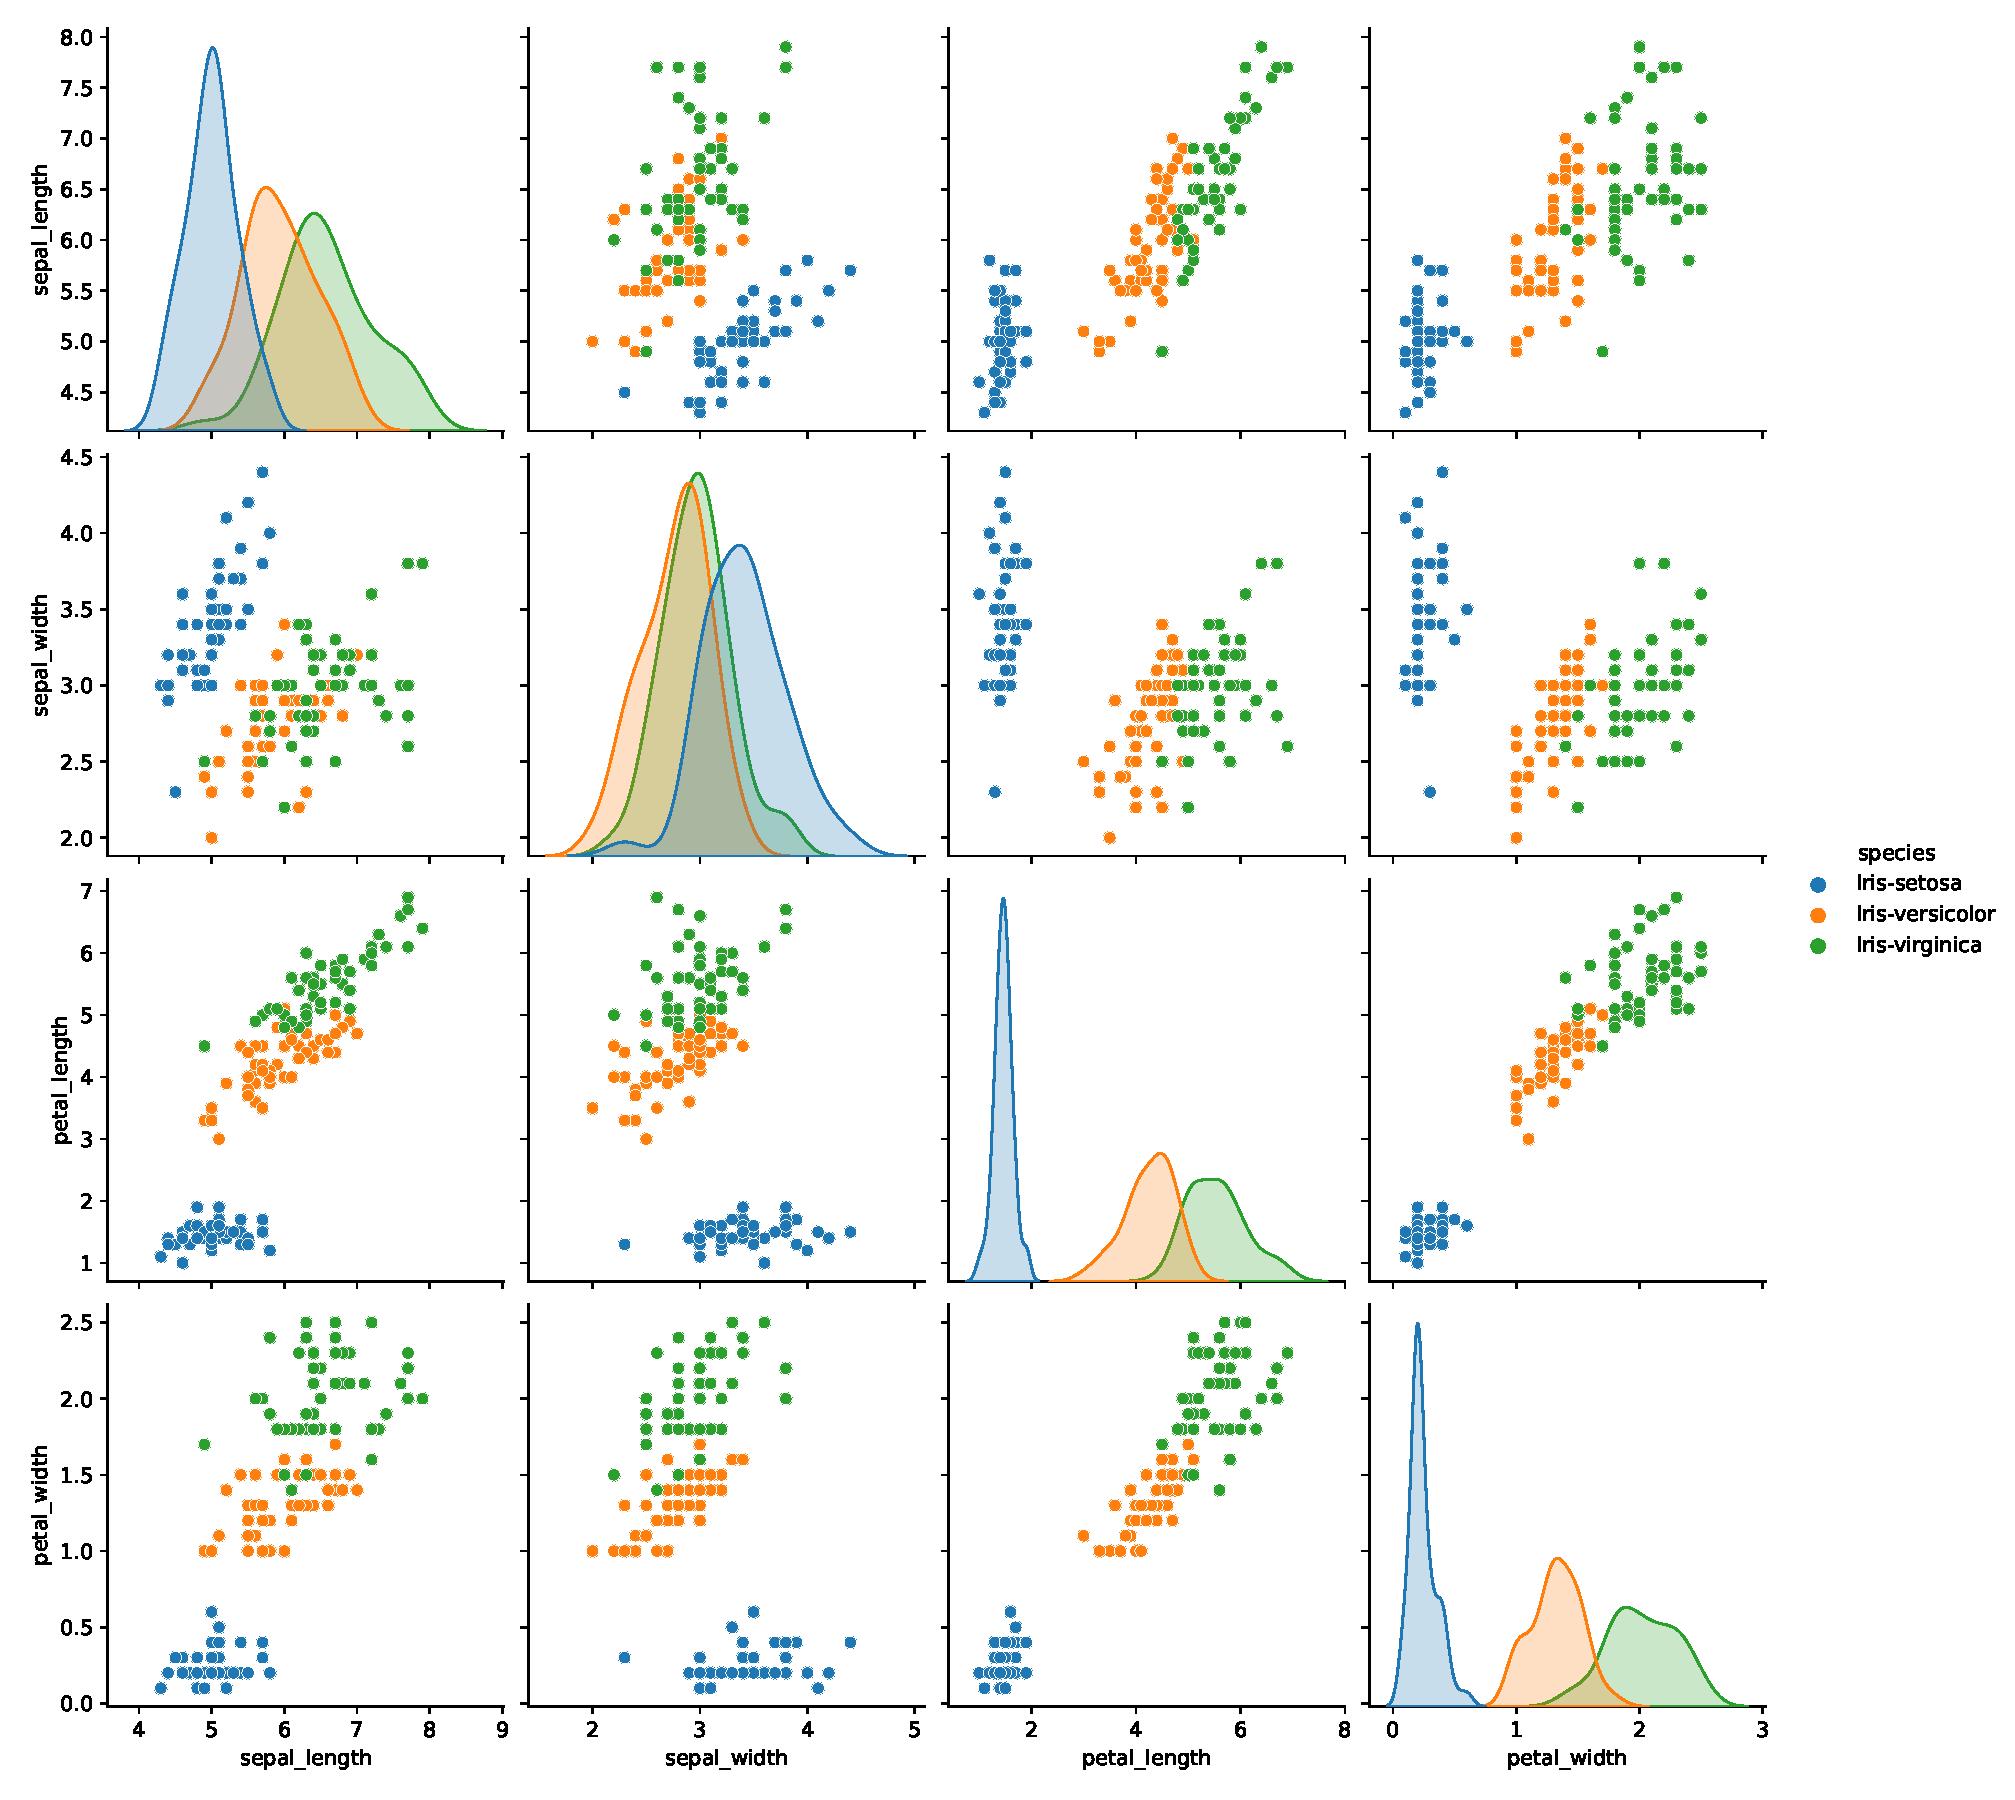
\includegraphics[scale=0.35]{../results/figures/figure.pdf}
\caption{Iris dataset}
\label{fig:iris}
\end{figure}

\section{Conclusion}
``I always thought something was fundamentally wrong with the universe'' \citep{adams1995hitchhiker}

\bibliographystyle{plain}
\bibliography{references}
\end{document}
